\documentclass[a4paper,12pt]{article}
\usepackage[MeX]{polski}
\usepackage[utf8]{inputenc}
\usepackage{graphicx}
%opening
\title{Marin Tufan}
\author{Marcel Mendziński}

\begin{document}

\maketitle

\tableofcontents
	
\begin{abstract}

\end{abstract}


\section{Marin Tufan}
	\begin{figure}[h]
	\centering
	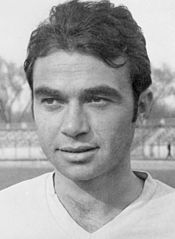
\includegraphics[width=0.25\hsize ]{foto/Marin_Tufan.jpg}
	\caption{Marin Tufan}\label{fig:Marin Tufan}
	\end{figure}
	
	Marin Tufan (ur. 16 października 1942 w Istrii) --- piłkarz rumuński grający na pozycji napastnika. Podczas kariery piłkarskiej mierzył 172 cm wzrostu, ważył 69 kg. W swojej karierze rozegrał 2 mecze w reprezentacji Rumunii.
	
\section{Kariera klubowa}
Karierę piłkarską Tufan rozpoczął w klubie Farul Konstanca. W 1963 roku awansował do kadry pierwszej drużyny. 15 września 1963 roku zadebiutował w pierwszej lidze rumuńskiej w przegranym 0:2 wyjazdowym meczu z UT Arad. Od czasu debiutu był podstawowym zawodnikiem Farulu. W Farulu grał do końca sezonu 1972--1973. ,,Największym jego sukcesem za czasów gry w Farulu było zajęcie 4. miejsca w lidze w sezonie 1966--1967, zarazem najwyższego w historii klubu. W barwach Farulu Tufan rozegrał 230 meczów i strzelił 62 gole.'' Jest najlepszym strzelcem w historii Farulu.

Latem 1973 roku Tufan przeszedł z Farulu do drugoligowego SC Tulcea. W 1976 roku spadł z nim z drugiej do trzeciej ligi. Po sezonie 1976--1977 zakończył karierę piłkarską.

	\begin{table}
		\begin{tabular}{ccccll}
			\hline
			\taxtbf{Sezon}&\taxtbf{Klub}&\taxtbf{Kraj}&\taxtbf{Rozgrywki}&\taxtbf{Mecze}&\taxtbf{Bramki}\\
			\hline
			
		\end{tabular}
	\end{table}
\end{document}